%% LyX 1.6.2 created this file.  For more info, see http://www.lyx.org/.
%% Do not edit unless you really know what you are doing.
\documentclass[english]{article}
\usepackage[T1]{fontenc}
\usepackage[latin9]{inputenc}
\usepackage{amsmath}

%%%%%%%%%%%%%%%%%%%%%%%%%%%%%% User specified LaTeX commands.

\author{Jordan T Dawe, Phil Austin}


\usepackage{babel}
\usepackage{graphicx}

\begin{document}

\title{Interpolation of LES cloud surfaces for use in direct calculations
of entrainment and detrainment}

\maketitle

\begin{abstract}
Direct calculations of the entrainment and detrainment of air between
clouds and their environment require a knowledge of the relative velocity
difference between the air and the cloud surface. LES model grids
force the distance moved by the cloud surface over a timestep to be
either zero or the width of a model grid cell, while in reality the
cloud surface tends to move at a more constant rate. Here we present
a method for the subgrid interpolation of a cloud surface given total
humidity and saturated humidity on a regular LES grid. This method
is used to calculate entrainment and detrainment rates for an LES
model, which are compared with rates inferred from bulk conserved
tracer calculations. 
\end{abstract}

\newpage

\section{Introduction}

The largest uncertainties in Global Circulation Model (GCM) simulations
come from the subgridscale parameterization of clouds. The IPCC 2007
report found the *TK* models they examined showed a *TK* W
m$^{-2}$ range in the cloud feedback response, relative to a *TK*
W m$^{-2}$ total climate sensitivity.  Improvements in the accuracy of 
these subgridscale cloud parametrizations are neccessary to simulate 
the rate and spatial pattern of global warming.

Proper simulation of the subgridscale effect of cumulus clouds in
GCMs requires understanding the rates at which air is entrained into
and detrained from the clouds. Cloud entrainment and detrainment rates
exert influences on profiles of cloud properties, the height of the
cloud tops, the amount of heat and moisture the clouds transport upwards,
and the heights at which the clouds deposit that heat and moisture.
They also have effects on the vertical transport of aerosols out of
the boundary layer and the rate at which chemical reactions can occur
in those aerosols. Several approaches to the parametrization of entrainment
and detrainment rates have been proposed, including *TK*.

Large Eddy Simulation (LES) is an important tool used in the study
of cloud entrainment and detrainment. LES models achieve grid resolutions
on the order of 10-100 m, so that the smallest length scales resolved
by the model touch the small wave number end of the Kolmagorov -5/3
turbulence spectrum. This allows for a relatively simple turbulence
model that captures the important statistics of the subgridscale eddy
fluxes and thus, an accurate representation of the atmospheric physics
of a domain \textasciitilde{}10 km$^{2}$, which is enough to simulate
a field of clouds. LES simulations can be ground-truthed against results
taken from large field surveys, such as the Barbados Oceanographic
and Meteorological Experiment (BOMEX) or the Atmospheric Radiation
Measurement (ARM) Program, and such comparisons show good agreement
between the LES simulations and field data.

Several recent studies have looked at the lifecycle of individual
clouds taken from LES models, trying to break the cloud field into
its component parts. Estimates of entrainment and detrainment rates
for individual clouds would be quite useful in these types of studies,
but are difficult to achieve. Entrainment and detrainment rates are 
typically calculated in LES simulations by recording budgets
of bulk conserved tracer variables, such as the total humidity or
the liquid water moist static energy, and inferring the amount of
fluid exchange between cloud and clear air that is needed to explain
the rate at which that tracer is being vertically advected within
the cloud field. These budgets typically assume the clouds and the
cloud environment are horizontally homogenous slabs; this is a much
less accurate assumption on the level of an individual cloud.

Alternatively, entrianment and detrianment could simply be calculated
directly from the LES velocity and humidity field.  \cite{Siebesma1998} 
defines Entrainment and Detrainment as

\begin{equation}
E = -\frac{1}{A}\oint_{\mathbf{\hat{n}}\cdot(\mathbf{u} - \mathbf{u_i}) < 0}
\mathbf{\hat{n}}\cdot(\mathbf{u}-\mathbf{u_i})dl
\end{equation}
\begin{equation}
D = \frac{1}{A}\oint_{\mathbf{\hat{n}}\cdot(\mathbf{u} - \mathbf{u_i}) > 0}
\mathbf{\hat{n}}\cdot(\mathbf{u}-\mathbf{u_i})dl
\end{equation}

where $E$ and $D$ are the entrainment and detrainment rates in kg 
m$^{-3}$ s$^{-1}$, u is velocity in m s$^{-1}$, *TK*.  However, the
accuracy of this method suffers from the need to calculate the velocity 
of the air relative to the cloud surface.  In reality 
these velocities are very nearly identical, \textasciitilde{} 1 m 
s$^{-1}$, but the discrete nature of the LES model grid forces the 
modeled surface velocity to be either 0 m s$^{-1}$ or $\Delta x / \Delta t 
\approx$ 30 m s$^{-1}$, where $\Delta x$ is the model grid spacing and 
$\Delta t$ is the model timestep.  The surface of the cloud only moves 
when a grid cell's humidity reaches saturation, and when it 
does, an entire grid cell worth of fluid leaves or enters the cloud.  This 
causes both the entrainment and detrainment to be over-estimated.

Here we present a method for calculation of the cloud entrainment and 
detrainment rates that relies on interpolation of the subgrid location 
of the cloud surface.  In section 2 we describe this method, in section 
3 we compare this calculation with entrainment and detrainment rates 
calculated using bulk conserved tracer budgets, and in section 4 we 
discuss our results.  With this method, we believe accurate estimates 
of the cloud entrainment and detrainment rates are possible for 
individual LES clouds.

\section{Method}

\subsection{Flux Calculations}

Consider a discrete 3-d numerical model operating on an Arakawa C-grid
(Fig \ref{fig:C_grid}) containing a cloud surface $\mathbf{A}$, where
the vectors representing $\mathbf{A}$ point outward from the cloud.  For 
the moment we neglect specifying the interpolation scheme that determines 
this surface.  This surface, combined with the walls of the grid cell, 
encloses a cloud volume $V$.  

Converted to our notation, \cite{Siebesma1998} gives the net Entrainment 
and Detrainment over the cloud interface to be:

\begin{equation}
\label{eq:E_minus_D} 
E - D = \int_A \rho ( \mathbf{u} -  \mathbf{u_i}) \cdot d\mathbf{A}.
\end{equation}

where $\rho$ is the air density in kg m$^{-3}$, $\mathbf{u}$ is the velocity
of the air in m s$^{-1}$ and $\mathbf{u_i}$ is the velocity of the cloud interface. 
Calculating this integral for a numerical model cloud field would require interpolation
of the velocity field to the surface of  $\mathbf{A}$ and a record of the time 
evoluion of $\mathbf{A}$.  Instead, we seek a simplified but equivalent calculation.

To calculate the velocity of the cloud interface, we make use of the Leibnitz Theorem:

\begin{equation}
\label{eq:leibnitz} 
\frac{d}{dt}\int_{V(t)} \rho dV = \int_{V(t)} \frac{\partial \rho}{ \partial t} dV 
                                + \int_{A(t)} \rho \mathbf{u_i}\cdot d\mathbf{A}
\end{equation}

Since the walls of the grid cell do not move, if we assume
${\partial \rho}/{ \partial t} \approx 0$ we can combine equations (\ref{eq:E_minus_D}) 
and (\ref{eq:leibnitz}) to give:

\begin{equation}
E - D = \rho \int_A \mathbf{u} \cdot d\mathbf{A} -  \rho \frac{d}{dt}\int_{V(t)} dV.
\end{equation}

Next we apply the divergence theorem to simplify the flux integral through $\mathbf{A}$:

\begin{equation}
\label{eq:divergence} 
\int_{V} \nabla \cdot (\rho \mathbf{u}) dV = \int_{A} \rho \mathbf{u}\cdot d\mathbf{A}
\end{equation}

Due to mass conservation, $\nabla \cdot (\rho \mathbf{u}) = 0$, which implies that
the massflux passing through $\mathbf{A}$ is equal to the massflux entering the volume $V$ 
through the walls of the model grid cell.  If we take the u and v velocities at the 
grid cell walls to be constant, we can calculate these fluxes simply by multiplying the 
velocity by the area of the grid cell wall occupied by cloud.  Thus:

\begin{equation}
E - D = \rho \int_S \mathbf{u} \cdot d\mathbf{S} -  \rho \frac{dV}{dt}
\end{equation}.

Thus, to calculate the entrainment and detrainment, we need to calculate the flux through 
the cloudy portion of the grid cell walls, and the rate of change of the cloud volume 
inside the grid cell.

\subsection{Cloud Surface Interpolation}

There are a multitude of interpolation schemes that can be used to determine the cloud 
volume and cell wall area in a numerical model.  The simplest would be to assume 
that saturated grid cells are completely filled with cloud and unsaturated grid cells 
have no cloud at all.  We refer to this as the "no inerpolation" case.

At the other end of the range of interpolation schemes, we can use linear (or higher order) 
interpolation to estimate the surface where the total water equals the saturated humidity 
and calculate the cloud volume and cell surface areas at each timestep.  Several standard 
techniques exist for this kind of calculation in the field of computer visualization, such
as the Marching Squares algorithm *TK*.  These techniques, however, are generally complex and 
require large amounts of calculation to perform.

Instead of these complex interpolation schemes, we propose a compromise scheme that calculates 
an approximate area and volume for the cloud surface while requiring much less computation time.
To do this, we divide each grid cell into six pyramids (Figure \ref{fig:pyramid_scheme}).  Next,
we compute the value of $q_{diff} = q_t - q_{sat}(T, p)$, which is positive for cloudy points and negative for 
clear points.  Then we compare the value of $q_{diff}$ with the nearest neighbour cells in all
six directions around the grid cell.  If both are clear, the pyramid contains no cloud and the 
area of cloud at the cell wall is zero.  If both are cloudy, the pyramid is filled with cloud 
and the cell wall is completely cloudy.  Otherwise, the fractional distances between the grid
cell centers at which $q_{diff} = 0$ is calculated via linear interpolation:

\begin{equation}
x = \frac{q_{diff}(1)}{q_{diff}(2) - q_{diff}(1)}
\end{equation}

This is taken to be the location of the cloud surface, and we assume the surface cuts the 
pyramid parallel to the grid cell wall.  Thus, if the cloud surface is outside the grid cell, 
the entire pyramid is set to be cloudy (or clear) and the grid cell wall area is set to be 
cloudy (or clear).  If the cloud surface is inside the grid cell, however, the volume of the 
cut pyramid is calculated as:

\begin{equation}
V = \frac{4}{3}x^3
\end{equation}

and the cell wall is set to clear (or cloudy, depending on the value of $q_{diff}$).

Finally, to calculate the flux through the cloud walls, we simply calculate the mass flux
through any cloudy grid cell wall using the model's continuity equation solver, and sum the 
flux for any cloudy grid cell wall.

We have implimented both the "no interpolation" and the "pyramid" schemes in the System 
for Atmospheric Modeling (SAM, \cite{Khairoutdinov2003}).  Running both schemes to calculate
entrainment and detrainment in a standard GCSSARM run (\cite{Brown2002}) shows that the 
"no interpolation" scheme estimates entrainment and detrainment rates to be double those 
estimated using the "pyramid" scheme (Figure \ref{fig:effect_of_interpolation}).

\section{Comparison with conserved bulk tracer calculations}

\cite{Siebesma1995} derive the following equations for entrainment and detrainment from a
simple entraining plume based on conserved bulk tracer properties:

\begin{equation}
  \begin{split}
    E (\chi_e - \chi_c) 
    = M_c \frac{\partial \chi_c}{\partial z}
    + \frac{\partial \rho a \overline{w' \chi'}^c}{\partial z} \\
    + \rho a \frac{\partial \chi_c}{\partial t}
    - a \rho \left(\frac{\partial \bar{\chi}}{\partial t}\right)_{forcing}
  \end{split}
\end{equation}

\begin{equation}
  \begin{split}
    D (\chi_e - \chi_c)
    = M_c \frac{\partial \chi_e}{\partial z}
    - \frac{\partial \rho (1 - a) \overline{w' \chi'}^e}{\partial z} \\
    - \rho (1 - a) \frac{\partial \chi_e}{\partial t}
    + \rho (1 - a) \left(\frac{\partial \bar{\chi}}{\partial t}\right)_{forcing}
  \end{split}
\end{equation}

Here $\chi$ represents any conserved bulk tracer, such as total water ($q_t$, kg kg$^{-1}$) or 
liquid water moist static energy ($h$, J kg$^{-1}$), $a$ is the fractional cloud area, $M_c$
is vertical mass flux, $w$ is vertical velocity in m s$^{-1}$.  $e$ and $c$ sub- and 
super-scripts denote values conditially sampled in the environemnt and cloud, primed values 
represent anomalies relative to the horizontal mean, and overbars represent horizontal 
averaging.  These equations form the basis of most calculations of entrainment and detrainment 
in the literature (*TK*).

Comparison of our direct entrainment scheme with Siebesma and Cuijper's bulk tracer method 
shows our method estimates values approximately 4 times larger than the bulk tracer method 
(Figure \ref{fig:direct_vs_tracer}.  There are several possible reasons for this.  First, 
Siebesma and Cuijper's method assumes the fluid being entrained and detrained has the mean 
properties of the environment and the clouds, respectively.  If the difference between the 
bulk tracer values near the cloud surface is smaller than the differences between the mean 
cloud and environment values, the bulk tracer calculation will underestimate $E$ and $D$.
Second, the bulk entrainment calculations assume that fluid that enters or leaves the clouds
does not depart or re-enter their original source within the averaging period.  The action of
small-scale turbulence could drive recirculations which increase the rate of $E$ and $D$ but 
do not significantly change the bulk tracer properties of the clouds.  We investiage each of
these possibilities in turn.

\subsection{Radial cloud structure}

\subsection{Strength of turbulent recirculations}

\subsection{Correlation of bulk tracer and direct calculation methods}

While we may have explained the difference in the magnitudes of the $E$ and $D$ values 
calculated, we still have not shown that large entrainments calculated using the bulk 
tracer method correspond to large entrainments in the direct method.  To do this, we take 
the correlation over the whole model run of the horizontally averaged $E$ and $D$ values
calculated via the two methods at each height to generate correlation profiles.  Time/Heights
where the model has no clouds are excluded from the calculation.  The result of this 
shows significant correlations between the methods for both $E$ and $D$ at all heights 
(Figure \ref{fig:correlations}).

\section{Discussion}

We have shows that using a simple interpolation scheme we have been able to calculate 
direct entrainment and detrainment rates that are more accurate than a scheme without 
interpolation and which are statistically consistent with entrainment and detrainment 
calculated using conserved bulk tracers.

-Discuss better interpolation schemes

-Probably still want to transform direct entrianment values into bulk entrainment values for
use in cloud parameterizaitons.

-However, it may be possible to improve the parameterizations with a relationship governing 
the ratio of direct to bulk tracer entrainment.

-Have to calculate bulk tracer entrainment and detrainment to calibrate the direct calculation
values

-Suitable for use in calculating entrainment and detrainment rates for individual clouds.



\section*{Acknowledgments}

Figures were generated using the matplotlib library in the Python
programming language.

\bibliographystyle{agu}

\bibliography{entrainment_interpolation}{} 

\newpage

\begin{figure}
\label{fig:C_grid}
\noindent\includegraphics{Figure1.eps} 
\caption{C grid cell with cloud surface.}
\end{figure}

\begin{figure}
\label{fig:pyramid_scheme}
\noindent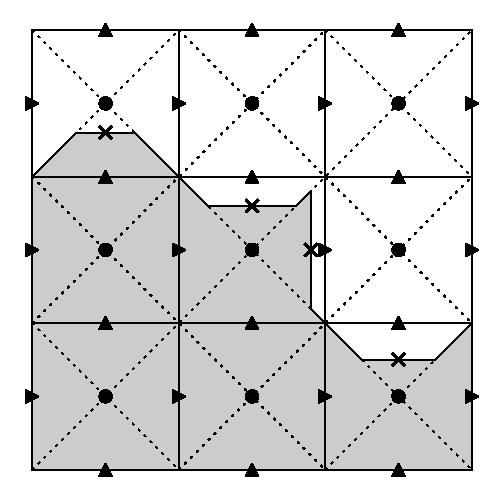
\includegraphics{Figure2.eps} 
\caption{Schematic representaiton of our pyramid interpolation scheme.}
\end{figure}

\begin{figure}
\label{fig:effect_of_interpolation}
\noindent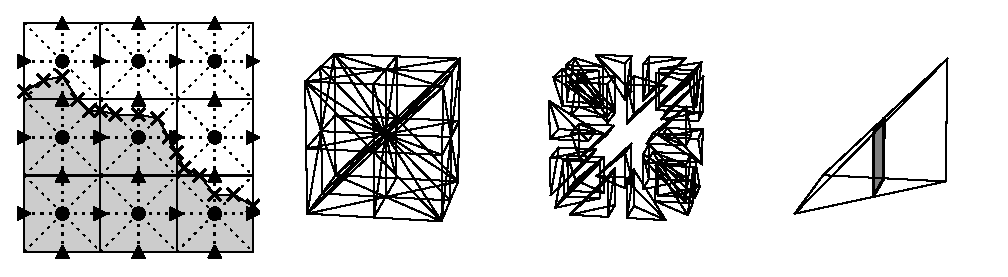
\includegraphics{Figure3.eps} 
\caption{Effect of surface interpolation on calculation of a) entrainment and b) detrainment.}
\end{figure}

\begin{figure}
\label{fig:direct_vs_tracer}
\noindent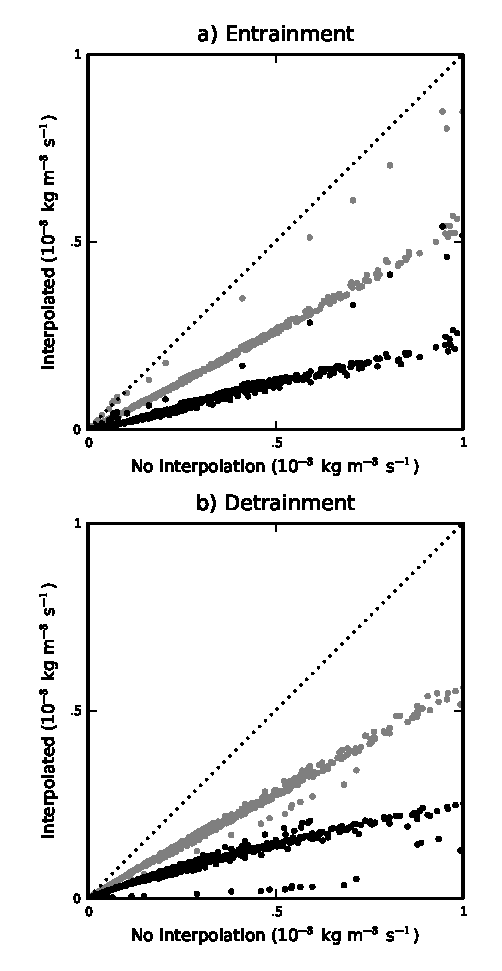
\includegraphics{Figure4.eps} 
\caption{Comparison of entrainment rates calculated using a) our direct method using pyramid 
interpolation, b) using the conserved bulk tracer method, and c) the ratio of the two methods.}
\end{figure}

\begin{figure}
\label{fig:entrainment_vs_radial_structure}
\noindent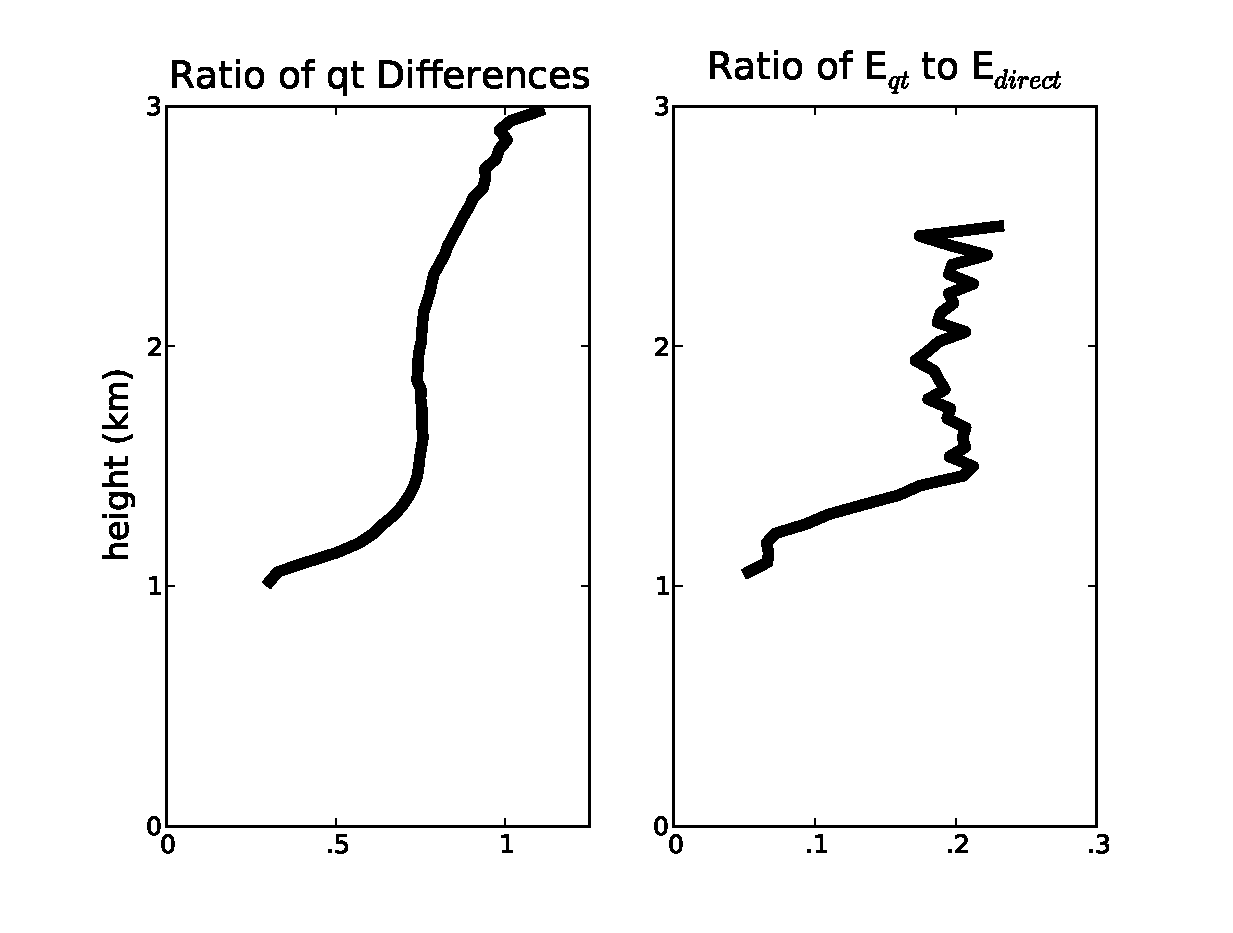
\includegraphics{Figure5.eps} 
\caption{Comparison of a) ratio of direct to tracer entrainment, and b) ratio of mean cloud-environment bulk tracer
differences to differences at the cloud edge.}
\end{figure}

\begin{figure}
\label{fig:resolution}
\caption{Dependance of direct entrainment on model grid resolution.}
\end{figure}

\begin{figure}
\label{fig:correlations}
\caption{Correlation between a) entrainment and b) detrainment calculated using conserved
bulk tracers and direct entrainment calculations with pyramid interpolation.}
\end{figure}

\end{document}
